% \vspace{-1mm}
\section{The Curse of Multilinguality---Model Capacity Constraints}
\label{sec:capacity}
% \vspace{-1mm}

\begin{figure*}
    \centering
    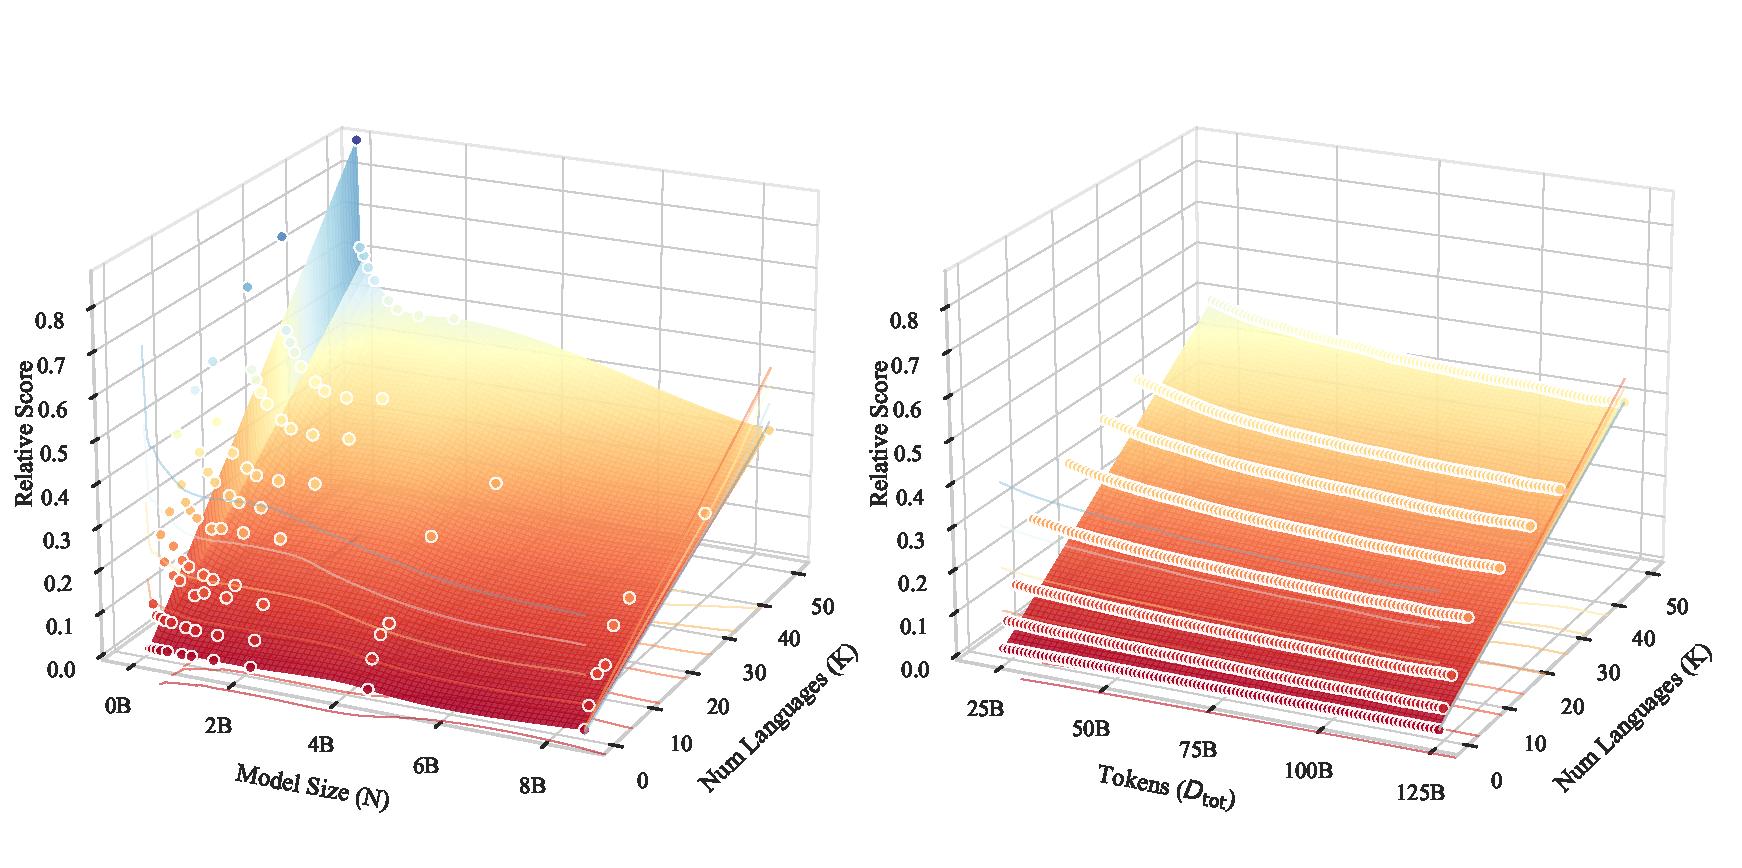
\includegraphics[width=0.92\textwidth]{figures/capacity/combined_capacity_contour.pdf}
    \vspace{-3mm}
    \caption{We empirically measure the relative degradation in loss (y-axis), as compared to a monolingual model of the same $(N,D)$, from adding pretraining languages (z-axis).
    \textbf{Left:} We fix $D=25B$ tokens, and vary the model size $N$.
    \textbf{Right:} We fix $N=2B$ parameters, and vary the tokens $D$. 
    The points are real empirical observations, averaged across languages. The mesh-grid is a surface estimate, using a cubic spline.
    \textbf{Target language loss is most affected by the number of training languages, but this loss penalty declines for larger models with more capacity.} 
    }
    \label{fig:capacity_surface_plot}
    % \vspace{-4mm}
\end{figure*}

\noindent\textbf{Research Question:} \emph{Is the ``curse of multilinguality'' measurable---the phenomenon where adding languages to the training mixture can degrade loss of each language, due to limited model capacity?}

A model's capacity can hinder its ability to learn multiple languages at once---known as the \emph{curse of multilinguality} \citep{conneau2019unsupervised, chang2024multilinguality}.
We can empirically measure this relationship, between $N$, $D$, and the number of training languages $K$, by running experiments with variable $K$.
Full experimental details and scaling law derivations are provided in \Cref{app:model-capacity-exp-details}.

% \vspace{-1mm}
\noindent\textbf{Modeling the Relationship between $K$, $N$, and $D$.} 
In \Cref{fig:capacity_surface_plot} we examine the relative loss increase, over a monolingual baseline, from varying the number of training languages $K$, and either the model size $N$ (left plot) or total training tokens $D_{\mathrm{tot}}$ (right plot).
For simplicity, we don't explicitly model token repetition, and we sample tokens from each language uniformly---we believe this is a reasonable assumption for models designed to serve all $K$ languages.
We observe three phenomena.
First, the number of training languages $K$ has far more impact on the relative loss than $N$ or $D$.
Relative loss appears to grow monotonically as $K$ increases.
Second, both increasing model size $N$ and total tokens $D_{\mathrm{tot}}$ mitigate this penalty.
However, computing the partial along the fitted surface shows $|\partial S/\partial\log N| > |\partial S/\partial\log D|$; indicating $N$ delivers larger marginal gains than $D_{\mathrm{tot}}$.
Consequently, maintaining performance as $K$ grows requires scaling both data and model size, but scaling the model size has a greater effect.
To understand the relationship among these variables more precisely, we model per--target--language loss as
\[
L(K,N,D_{t})\;=\;L_\infty \;+\; A\,\frac{K^{\phi}}{N^{\alpha}}
\;+\; B\,\frac{K^{\psi}}{D_{t}^{\beta}},
\]
where, under even sampling the total tokens across languages are \(D_{\mathrm{tot}} = K\,D_{t}\).
We tested several scaling law variations for this research question, but settled on this one as (a) it retains Chinchilla-style power-law decay properties that cleanly separate model capacity from data (it also reduces to Chinchilla when K=1), (b) it makes the role of the number of languages explicit and interpretable, and (c) it achieved a robust $R^2\ge0.87$, indicating a strong fit.
The exponent \(\phi\) captures how capacity requirements grow with the number of languages, while \(\psi\) captures how data requirements change with multilinguality. \(\psi<0\) indicates \emph{positive transfer} (sublinear data needs per language as \(K\) increases), and \(\psi>0\) implies negative transfer/interference.

% \begin{wrapfigure}{l}{0.5\textwidth}
%     \centering
%     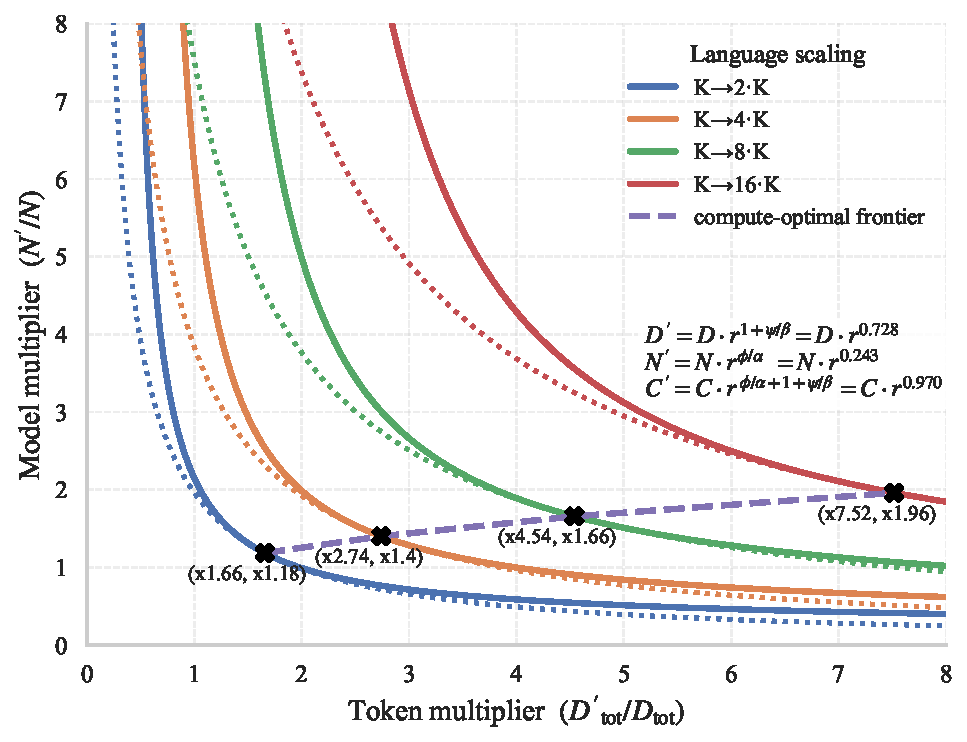
\includegraphics[width=0.48\textwidth]{figures/capacity/capacity_add_lang_pareto_curve_v2.pdf}
%     \caption{
%     \textbf{Iso-loss from expanding language coverage: }
%     When scaling the number of languages a model serves from $K \rightarrow r \cdot K$, we can estimate how much they need to increase model size $N'/N$ and/or training tokens $D'_{tot}/D_{tot}$, without degrading any of their languages' loss. 
%     We derive the compute optimal scaling equations. 
%     \textbf{The \emph{iso-losses} indicate that a practitioner should expand their compute budget by $C \cdot r^{0.97}$ to expand their language coverage by $r$.}\label{fig:capacity_add_lang_isoloss_curve}
%     }
% \end{wrapfigure}

\begin{wrapfigure}{L}{0.5\textwidth}
    \centering
    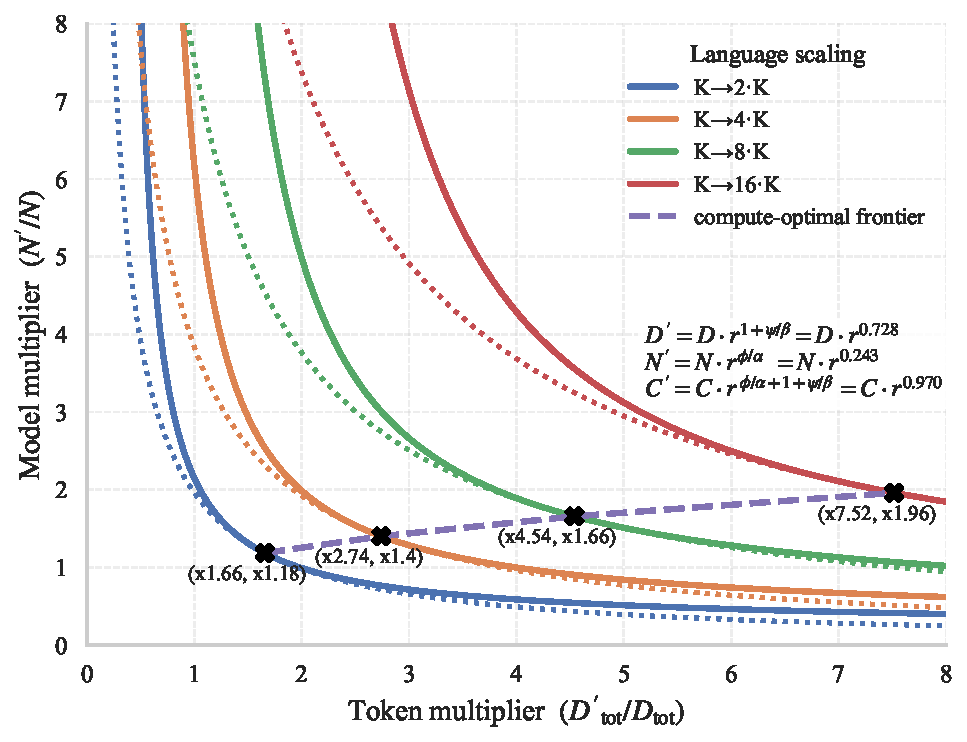
\includegraphics[width=0.48\textwidth]{figures/capacity/capacity_add_lang_pareto_curve_v2.pdf}
    \caption{
    \textbf{Iso-loss from expanding language coverage: }
    When scaling the number of languages a model serves from $K \rightarrow r \cdot K$, we can estimate how much they need to increase model size $N'/N$ and/or training tokens $D'_{tot}/D_{tot}$, without degrading any of their languages' loss. 
    We derive the compute optimal scaling equations. 
    \textbf{The \emph{iso-losses} indicate that a practitioner should expand their compute budget by $C \cdot r^{0.97}$ to expand their language coverage by $r$.}\label{fig:capacity_add_lang_isoloss_curve}
    }
\end{wrapfigure}


We fit the scaling law for each of 8 different languages, as well as the combination of all, achieving similar coefficients, and $>0.8$ $R^2$ for each.
Using the scaling law fit on all language data we find \(\phi=0.11\) and \(\psi=-0.04\), indicating a mild capacity-driven curse of multilinguality, tempered by positive transfer across languages.
In other words, as languages are added to the training mixture, a positive $\phi$ means the loss will decline from limited model capacity, however, a negative $\psi$ means that \textbf\emph{{less data per language is needed.}}
(Though the total amount of data increases, as we sample from new languages too.)
This provides clear, measurable evidence of positive cross-lingual transfer.


\noindent\textbf{Estimating the Iso-Loss Frontier, and Compute-Optimal scaling of $N,D$ when adding languages: $K\rightarrow rK$.} 
% \paragraph{Iso--loss frontier and compute--optimal scaling.}
Next, we examine the practical case where a practitioner wants to retrain a new model, increasing the number of languages it serves from $K$ to $rK$, without hindering the performance the original model achieved on the existing languages.
To accommodate these new languages, they will need to scale $C$ with some combination of $N\rightarrow N'$ and $D_{\mathrm{tot}}\rightarrow D_{\mathrm{tot}}'$.
We can compute this iso-loss by equating the loss terms: $L(K,N,D_{\mathrm{tot}}) = \frac{A K^{\phi}}{N^{\alpha}} + \frac{B K^{\psi}}{D^{\beta}} = \frac{A (K r)^{\phi}}{N'^{\alpha}} + \frac{B (K r)^{\psi}}{D'^{\beta}}$. 
From this we can derive the closed-form expression for how to scale ($N,D_{\mathrm{tot}}$) when increasing $K$ to $rK$ (as derived in \Cref{app:model-capacity-exp-details}):
\[
\frac{N^{*}(rK)}{N^{*}(K)} \;=\; r^{\phi/\alpha},
\qquad
\frac{D_t^{*}(rK)}{D_t^{*}(K)} \;=\; r^{\psi/\beta},
\qquad
\frac{D_{\mathrm{tot}}^{*}(rK)}{D_{\mathrm{tot}}^{*}(K)} \;=\; r^{\,1+\psi/\beta}.
\]
We can also derive the minimal increase in the compute budget:
\[
\frac{C'}{C}
\;=\;
\frac{N' D_{tot}'}{N D_{tot}}
\;=\;
\Bigl(\tfrac{N'}{N}\Bigr)^\star
\Bigl(\tfrac{D'_{\mathrm{tot}}}{D_{\mathrm{tot}}}\Bigr)^\star = r^{1+\phi/\alpha+\psi/\beta}\,.
\]
In \Cref{fig:capacity_add_lang_isoloss_curve} we plot the iso-loss frontiers, and compute-optimal allocations, when scaling a model from $K$ to $r \cdot K$ languages.
It shows in closed-form how a practitioner should scale $D_{tot}$, $N$, and by extension their compute budget $C$ to accommodate additional languages, without degrading their loss.
For instance, we find expanding to $4 \cdot K$ languages requires a practitioner to expand $D_{tot}$ by 2.74, and the model size $N$ by 1.4.
Incidentally, evenly sampling across languages, this actually corresponds to using sampling $1-(2.74/4)=32\%$ less data per language.
Although there are fewer tokens in each target language (by 32\%), the total tokens has risen by 2.74, and the positive transfer prevents any potential loss degradation.

